\documentclass[12pt]{article}

\usepackage{amsmath}
\usepackage{amssymb}
\usepackage{graphicx}

\counterwithin*{equation}{section}
\counterwithin*{equation}{subsection}

\graphicspath{ {./images/} } 

\begin{document}
\section{Curves in Polar Coordinates}
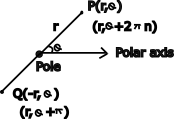
\includegraphics{polarcoordinates}\\%
Polar coordinates are constructed by the distance from the origin $a$ (radius) and the angle $\theta$.\\%
Previously, we used \underline{Rectangular Coordinates}\\%
\underline{Conversions}\\%
$x=r\cos\theta$\\%
$y=r\sin\theta$\\%
$\tan\theta=\frac{y}{x}$

\subsection{Example Polar 1}
\underline{Ex:} Convert $(r,\theta)=(2,\frac{\pi}{3})$ to Cartesian coordinates.

\begin{align}
	x=r \cos\theta, y=r \sin\theta\\%
	x=2 \cos \frac{\pi}{3}, y=2 \sin \frac{\pi}{3}\\%
	x=1, y=\sqrt{3}
\end{align}

\subsection{Example Polar 5}
\underline{Graph:} $r=\sin2\theta$\\%
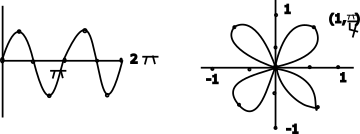
\includegraphics{flowerpolar}

\section{Parametric Equations}
\underline{Recall:} Parametric Equations\\%
if $r=f(\theta)$, then:\\%
$x=r\cos\theta = f(\theta)\cos\theta$\\%
$y=r\sin\theta=f(\theta)\sin\theta$

\subsection{Parametrc Example 1}

\subsection{Parametric Example 2}
Find  values of $\theta$ where the tangent line is horizontal or vertical.\\%
\underline{Hor:} $\frac{dy}{dx}=0=\frac{\frac{dy}{d\theta}}{\frac{dx}{d\theta}}$

\end{document}


